% This file was created by matlab2tikz.
%
%The latest updates can be retrieved from
%  http://www.mathworks.com/matlabcentral/fileexchange/22022-matlab2tikz-matlab2tikz
%where you can also make suggestions and rate matlab2tikz.
%
\definecolor{mycolor1}{rgb}{0.00000,0.44700,0.74100}%
\definecolor{mycolor2}{rgb}{0.92900,0.69400,0.12500}%
\definecolor{mycolor3}{rgb}{0.46600,0.67400,0.18800}%
\definecolor{mycolor4}{rgb}{0.63500,0.07800,0.18400}%
\definecolor{mycolor5}{rgb}{0.85000,0.32500,0.09800}%
%
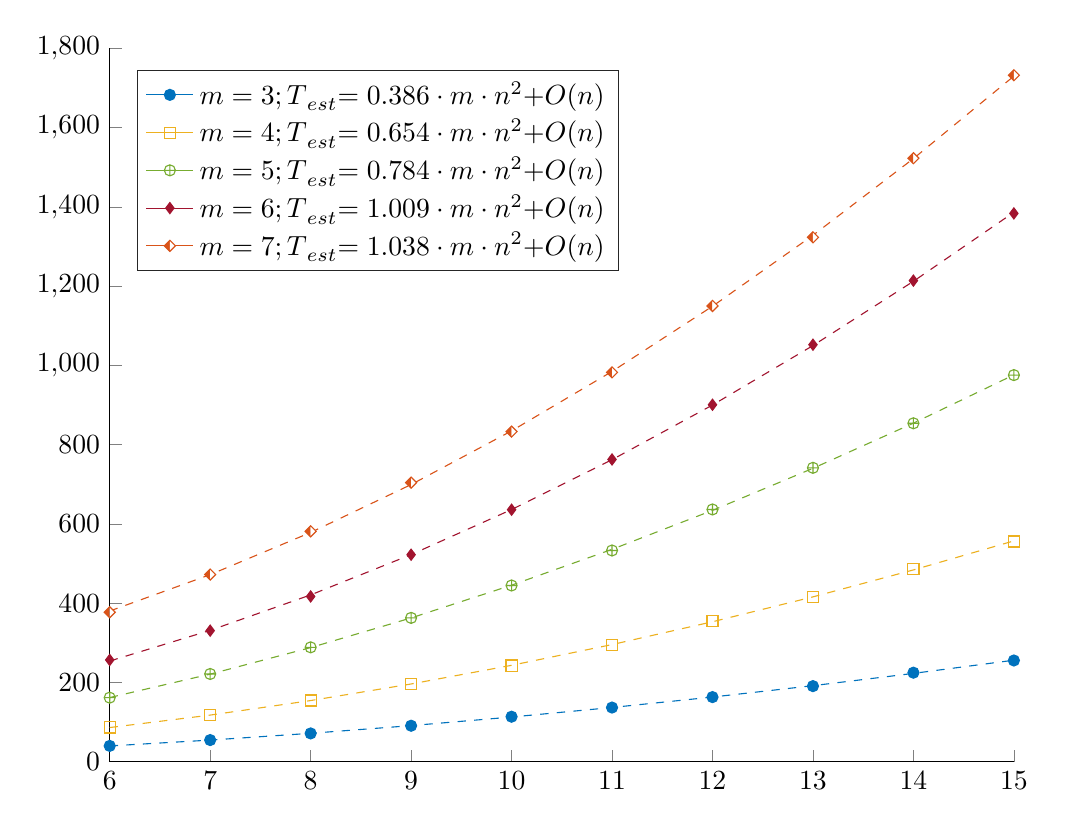
\begin{tikzpicture}

\begin{axis}[%
width=4.521in,
height=3.566in,
at={(0.758in,0.481in)},
scale only axis,
xmin=6,
xmax=15,
xlabel style={font=\color{white!15!black}},
%xlabel={n (row number)},
ymin=0,
ymax=1800,
ylabel style={font=\color{white!15!black}},
%ylabel={Time},
axis background/.style={fill=white},
title style={font=\bfseries},
% title={$\text{Average ticks until solution as a function of n. On n }\times\text{ m grid. (k = 5)}$},
axis x line*=bottom,
axis y line*=left,
legend style={at={(0.03,0.97)}, anchor=north west, legend cell align=left, align=left, draw=white!15!black}
]
\addplot [color=mycolor1, draw=none, mark=*, mark options={solid, mycolor1}]
  table[row sep=crcr]{%
6	39.87\\
7	54.6\\
8	71.374\\
9	90.742\\
10	113.546\\
11	136.656\\
12	163.044\\
13	190.74\\
14	224.654\\
15	255.43\\
};
\addlegendentry{$\text{m = 3; T}_{\text{est}}\text{ = 0.386 }\cdot \text{m} \cdot \text{n}^\text{2}\text{ + O(n)}$}

\addplot [color=mycolor1, dashed, forget plot]
  table[row sep=crcr]{%
6	39.7778545454546\\
7	54.548303030303\\
8	71.6371454545454\\
9	91.0443818181818\\
10	112.770012121212\\
11	136.814036363636\\
12	163.176454545455\\
13	191.857266666667\\
14	222.856472727273\\
15	256.174072727273\\
};
\addplot [color=mycolor2, draw=none, mark=square, mark options={solid, mycolor2}]
  table[row sep=crcr]{%
6	86.474\\
7	117.85\\
8	154.456\\
9	195.29\\
10	242.642\\
11	294.888\\
12	354.16\\
13	416.606\\
14	485.398\\
15	555.786\\
};
\addlegendentry{$\text{m = 4; T}_{\text{est}}\text{ = 0.654 }\cdot \text{m} \cdot \text{n}^\text{2}\text{ + O(n)}$}

\addplot [color=mycolor2, dashed, forget plot]
  table[row sep=crcr]{%
6	86.2083636363648\\
7	117.624303030303\\
8	154.271484848485\\
9	196.149909090909\\
10	243.259575757575\\
11	295.600484848484\\
12	353.172636363636\\
13	415.97603030303\\
14	484.010666666667\\
15	557.276545454546\\
};
\addplot [color=mycolor3, draw=none, mark=oplus, mark options={solid, mycolor3}]
  table[row sep=crcr]{%
6	161.644\\
7	221.38\\
8	288.6\\
9	362.958\\
10	444.712\\
11	533.07\\
12	636.62\\
13	741.686\\
14	854.076\\
15	975.69\\
};
\addlegendentry{$\text{m = 5; T}_{\text{est}}\text{ = 0.784 }\cdot \text{m} \cdot \text{n}^\text{2}\text{ + O(n)}$}

\addplot [color=mycolor3, dashed, forget plot]
  table[row sep=crcr]{%
6	161.895054545448\\
7	221.023660606058\\
8	287.991418181819\\
9	362.79832727273\\
10	445.444387878792\\
11	535.929600000004\\
12	634.253963636367\\
13	740.41747878788\\
14	854.420145454544\\
15	976.261963636359\\
};
\addplot [color=mycolor4, draw=none, mark=diamond*, mark options={solid, mycolor4}]
  table[row sep=crcr]{%
6	256.79\\
7	330.746\\
8	417.06\\
9	522.352\\
10	635.976\\
11	762.868\\
12	900.878\\
13	1052.474\\
14	1214.118\\
15	1383.794\\
};
\addlegendentry{$\text{m = 6; T}_{\text{est}}\text{ = 1.009 }\cdot \text{m} \cdot \text{n}^\text{2}\text{ + O(n)}$}

\addplot [color=mycolor4, dashed, forget plot]
  table[row sep=crcr]{%
6	254.020327272734\\
7	331.432569696972\\
8	420.95566060606\\
9	522.589599999997\\
10	636.334387878784\\
11	762.19002424242\\
12	900.156509090906\\
13	1050.23384242424\\
14	1212.42202424243\\
15	1386.72105454546\\
};
\addplot [color=mycolor5, draw=none, mark=halfsquare left*, mark options={solid, mycolor5}]
  table[row sep=crcr]{%
6	377.246\\
7	472.358\\
8	581.354\\
9	704.34\\
10	833.164\\
11	982.628\\
12	1150.17\\
13	1323.426\\
14	1523.172\\
15	1732.586\\
};
\addlegendentry{$\text{m = 7; T}_{\text{est}}\text{ = 1.038 }\cdot \text{m} \cdot \text{n}^\text{2}\text{ + O(n)}$}

\addplot [color=mycolor5, dashed, forget plot]
  table[row sep=crcr]{%
6	380.223072727265\\
7	472.09096363636\\
8	578.493506060606\\
9	699.430700000003\\
10	834.902545454549\\
11	984.909042424247\\
12	1149.45019090909\\
13	1328.52599090909\\
14	1522.13644242424\\
15	1730.28154545454\\
};
\end{axis}
\end{tikzpicture}%
